\documentclass[11pt,letterpaper]{article}
\usepackage[utf8]{inputenc}
\usepackage{amsmath}
\usepackage{amsfonts}
\usepackage{amssymb}
\usepackage{graphicx}
\usepackage{booktabs}
\usepackage{subcaption}
\usepackage{graphicx}
\usepackage{cite}
\usepackage[colorlinks = true,
            linkcolor = blue,
            urlcolor  = blue,
            citecolor = blue,
            anchorcolor = blue]{hyperref}
\usepackage[section]{placeins}
\usepackage{float}
\usepackage[left=2cm,right=2cm,top=2cm,bottom=2cm]{geometry}
\author{Tyler Folkman and Devesh Sahu}
\title{CS 384G Computer Graphics, Spring 2016 \\ Project Proposal}
\begin{document}
\maketitle

For our project, we plan on implementing a learning based method for processing grayscale photos. A recent method developed by Zhang, Isola, and Efros~\cite{zhang2016colorful} demonstrates a fully automatic method that colors a grayscale image with plausible colors. This is accomplished by leveraging convolutional neural networks to learn from data how an image could be colored. Our plan is to re-create this method and develop an app that allows users to take or upload an image and receive back the colored version. This project idea most resembles the image processing we did in the Impressionist homework.

From this project we hope to gain a better understanding of how learning based methods are used in computer graphics. Machine learning has been used in numerous graphics applications~\cite{grochow2004style}~\cite{barbivc2004segmenting}~\cite{matusik2003data} and convolutional neural networks have been making large gains in the computer vision area. We believe this project will help us see how these type of image networks can be leveraged in the field of computer graphics. 

We intend to produce an android application as our result that will perform this automatic coloring of grayscale images. The application will send the photo to a remote server that will run the neural network to produce the color version. We plan on working on most of the project together (pair programming). The steps in achieving this include developing the code for the convolutional neural network, initialize the weights using pre-trained data from the authors, creating code to evaluate a new grayscale image on the neural network, and create an android application that serves as the front end and communicates with our remote server. Below are examples of results provided by the authors:
\newline
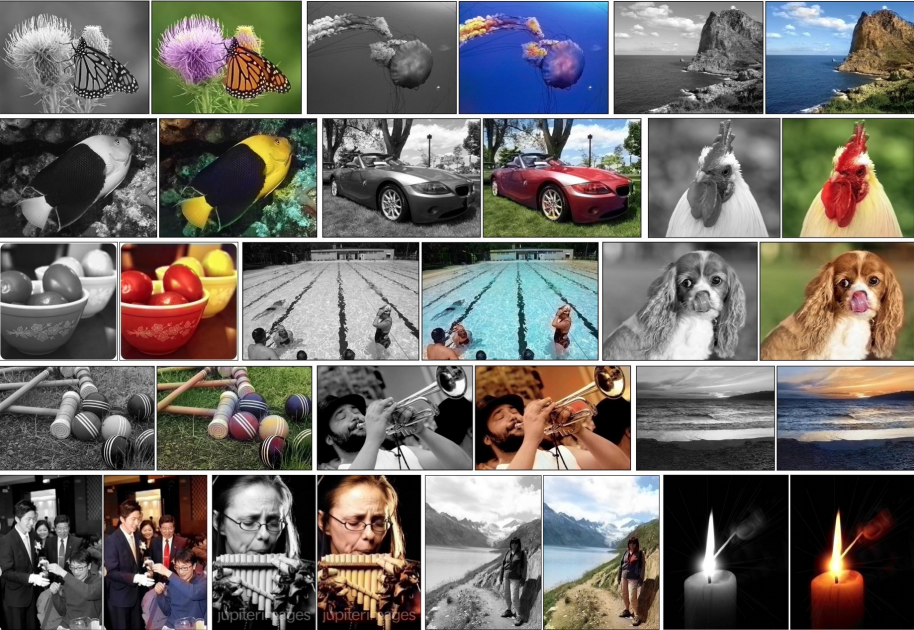
\includegraphics[scale=0.4]{color_examples.png}




\bibliography{mybib}
\bibliographystyle{plain}
\end{document}
